\documentclass{article}
\usepackage{amssymb,amsmath, verbatim}
%\usepackage{titlesec}  
\usepackage{epsfig}
%\usepackage{placeins}
\usepackage[margin=2cm]{geometry}
%\usepackage{fancyhdr}
%\pagestyle{fancy}
%\renewcommand{\headrulewidth}{0pt}
%\renewcommand{\footrulewidth}{1pt}

\usepackage{graphicx, float}
\usepackage[T1]{fontenc}
\usepackage{listings}
\usepackage{bm}

%\usepackage{names}

\DeclareMathOperator*{\argmax}{\arg\!\max}
\DeclareMathOperator*{\argmin}{\arg\!\min}

\newcommand{\pdiff}[2]{
        \frac{\partial #1}{\partial #2}
}

\newcommand{\diff}[2]{
        \frac{d #1}{d #2}
}


% Footer
%\lfoot{\thepage}
%\rfoot{\vspace{-.8cm} Michael Stewart, Andrea Corredor, Elahe Rahimtoroghi
%\\\vspace{.14cm}
%\footnotesize mijstewa@ucsc.edu, acorredo@ucsc.edu, elahe@soe.ucsc.edu}


                 
%\titleformat{\subsection}[runin]{}{}{}{}[] % makes subsections not appear on their own lines


%Header
\newcommand{\header}[5]{
        \begin{minipage}[h!]{0.63\textwidth}
                \centering
                { \LARGE \textbf{ \textsc{#1} } }
        \end{minipage}
        \begin{minipage}[h!]{0.37\textwidth}
                \centering
                {#2}\\
                {#3}\\
        \end{minipage}
}

\begin{document}

\header{Machine Learning HW \#3}
       {Michael Stewart\\Andrea Corredor\\Elahe Rahimtoroghi\\
       \{mijstewa, acorredo, elahe\}@ucsc.edu}
       {11/5/2013}
\\\\


\section{Decision Trees}

\subsection*{a: Pure children}
The right child is pure because all its data points belong to the same class (all have label 1).

\subsection*{b: Impurity if $x_2$ at the left node}
\begin{align*}
\text{Average impurity} = \frac{\left( n_1 \text{impurity}(p_1) + n_2 \text{impurity}(p_2) \right)}{n} \\
\text{impurity}(p) = 2p(1-p) \\  
\text{Let } n_1 \text{correspond to } x_2 = 0 \text{ and } n_2 \text{ to } x_2 = 1 \\
n1 = 2 \\
p1 = 1/2 \\
n2 = 2 \\
p2 = 1/2 \\
n = 4 \\
\text{Average impurity} = \frac{\left( 2*2*\frac{1}{2}\frac{1}{2}  + 2*2* \frac{1}{2}\frac{1}{2} \right)}{4} \\
\text{Average impurity} = \frac{1}{2}
\end{align*}
\subsection*{c: Impurity if $x_3$ at root}
\begin{align*}
\text{Let } n_1 \text{correspond to } x_3 = 0 \text{ and } n_2 \text{ to } x_3 = 1 \\
n1 = 1 \\
p1 = 1 \\
n2 = 3 \\
p2 = 1/3 \\
n = 4 \\
\text{Average impurity} = \frac{\left( 1*2*1*0  + 3*2* \frac{1}{3}\frac{2}{3} \right)}{4} \\
\text{Average impurity} = \frac{1}{3}
\end{align*}

\section{Artifical Neural Network}
Assume that the nodes do not have bias terms, and the initial weights are all $0$'s. \\
$\eta = 0.1$, training example $x_1 = 1, x_2 =2, t=1$. Show the $a_i,z_i$ and $\delta_i$ values for each non-input node, and the new weights after the backprop update.
\subsection*{Backpropagation with logistic sigmoid}
Going forward to compute all $a_j$ and $z_j$: \\
$x_1 = a_1 = z_1 = 1,~~x_2 = a_2 = z_2 =  2$ \\
$a_3 = \sum_{i=1}^{2} w_{3i} z_{i} =  0*1 + 0*2 = 0   $ \\
$z_3 = \sigma(a_3) = \frac{1}{1 + e^0} = \frac{1}{2}$ \\
$a_4 = \sum_{i=1}^{2} w_{4i} z_{i} =  0*1 + 0*2 = 0   $ \\
$z_4 = \sigma(a_4) = \frac{1}{2}$ \\
$a_5 = \sum_{i=3}^{4} w_{5i} z_{i} =  0*\frac{1}{2} + 0*\frac{1}{2} = 0   $ \\
$z_5 = a_5 = 0$ \\
\\
Computing $\frac{\partial E}{\partial a_k}$ at the output node: \\
$\frac{\partial E}{\partial a_{5}} = \left( a_5 - t \right) = (0 - 1) = -1$ \\
\\
Using Equation (5) to compute the other $\frac{\partial E}{\partial a_j}$ , working backwards through the network: \\
\begin{align*}
\frac{\partial E}{\partial a_j} = \left( \sum_{k \in U_j} \frac{\partial E}{\partial a_k} w_{kj}  \right) z_j (1-z_j)
\end{align*}
\begin{align*}
\frac{\partial E}{\partial a_4} &= \left( \frac{\partial E}{\partial a_5}*w_{5,4} \right)z_4(1-z_4) \\
&= (-1*0)*0.5*0.5 \\
&= 0
\end{align*}
\begin{align*}
\frac{\partial E}{\partial a_3} &= \left( \frac{\partial E}{\partial a_5}*w_{5,3} \right)z_3(1-z_3) \\
&= (-1*0)*0.5*0.5 \\
&= 0
\end{align*}
Thus, we find $\delta_4 = 0,~\delta_3 = 0$
\\
Using Equation (6) to compute the derivative of the error with respect to each weight in the network: \\
\begin{align*}
\frac{\partial E}{\partial w_{ji}} &= \delta_j z_i \tag{6} \\
\frac{\partial E}{\partial w_{5,3}} &= \delta_5 z_3 = -1*\frac{1}{2} = -\frac{1}{2} \\
\frac{\partial E}{\partial w_{5,4}} &= \delta_5 z_4 = -1*\frac{1}{2} = -\frac{1}{2} \\
\frac{\partial E}{\partial w_{3,1}} &= \delta_3 z_1 = 0*1 = 0 \\
\frac{\partial E}{\partial w_{3,2}} &= \delta_3 z_2 = 0*2 = 0 \\
\frac{\partial E}{\partial w_{4,1}} &= \delta_4 z_1 = 0*1 = 0 \\
\frac{\partial E}{\partial w_{4,2}} &= \delta_4 z_2 = 0*2 = 0
\end{align*}
\\
\\
Finally, update each $w_{ji}$ weight to $w{ji} - \eta \frac{\partial E}{\partial w_{ji}}$ where $\eta$ is the learning rate:
\begin{align*}
 w_{5,3} &= w_{5,3} - 0.1*-\frac{1}{2} = 0.05\\
 w_{5,4} &= w_{5,4} - 0.1*-\frac{1}{2} = 0.05\\
 w_{3,1} &= w_{5,3} - 0.1*0 = 0\\
 w_{3,2} &= w_{5,3} - 0.1*0 = 0\\
 w_{4,1} &= w_{5,3} - 0.1*0 = 0\\
 w_{4,2} &= w_{5,3} - 0.1*0 = 0\\
\end{align*}


\subsection*{Backpropagation with hyperbolic tangent sigmoid}
Now $\sigma(a) = tanh(a)$, which changes equation (5) as the derivative of $\frac{z_j}{a_j}$ is now $1 - \sigma(a)^2$. Since Eq (6) depends on Eq (5), the former also changes. 
The updated equations are:
\begin{align*}
\frac{\partial E}{\partial a_j} &= \delta_j = \left( \sum_{k \in U_j} \frac{\partial E}{\partial a_k} w_{kj}  \right) \left( 1 - z_j^2 \right) \tag{5} \\
\frac{\partial E}{\partial w_{ji}} &= \delta_j z_i  \tag{6}
\end{align*}

Going forward to compute all $a_j$ and $z_j$: \\
$x_1 = a_1 = z_1 = 1,~~x_2 = a_2 = z_2 =  2$ \\
$a_3 = \sum_{i=1}^{2} w_{3i} z_{i} =  0*1 + 0*2 = 0   $ \\
$z_3 = \sigma(a_3) = \frac{e^0 - e^0}{e^0 + e^0} = 0$ \\
$a_4 = \sum_{i=1}^{2} w_{4i} z_{i} =  0*1 + 0*2 = 0   $ \\
$z_4 = \sigma(a_4) = 0 $ \\
$a_5 = \sum_{i=3}^{4} w_{5i} z_{i} =  0*0 + 0*0 = 0   $ \\
$z_5 = a_5 = 0$ \\
\\
Computing $\frac{\partial E}{\partial a_k}$ at the output node: \\
$\frac{\partial E}{\partial a_{5}} = \left( a_5 - t \right) = (0 - 1) = -1$ \\
\\
Using Equation (5) to compute the other $\frac{\partial E}{\partial a_j}$ , working backwards through the network: \\
\begin{align*}
\frac{\partial E}{\partial a_j} = \left( \sum_{k \in U_j} \frac{\partial E}{\partial a_k} w_{kj}  \right)(1-z_j^2)
\end{align*}
\begin{align*}
\frac{\partial E}{\partial a_4} &= \left( \frac{\partial E}{\partial a_5}*w_{5,4} \right)(1-z_4^2) \\
&= (-1*0)*(1-0) \\
&= 0
\end{align*}
\begin{align*}
\frac{\partial E}{\partial a_3} &= \left( \frac{\partial E}{\partial a_5}*w_{5,3} \right)(1-z_3^2) \\
&= (-1*0)*(1-0)\\
&= 0
\end{align*}
Thus, we find $\delta_4 = 0,~\delta_3 = 0$
\\
Using Equation (6) to compute the derivative of the error with respect to each weight in the network: \\
\begin{align*}
\frac{\partial E}{\partial w_{ji}} &= \delta_j z_i \tag{6}\\
\frac{\partial E}{\partial w_{5,3}} &= \delta_5 z_3 = -1*0 = 0 \\
\frac{\partial E}{\partial w_{5,4}} &= \delta_5 z_4 = -1*0 = 0 \\
\frac{\partial E}{\partial w_{3,1}} &= \delta_3 z_1 = 0*1 = 0 \\
\frac{\partial E}{\partial w_{3,2}} &= \delta_3 z_2 = 0*2 = 0 \\
\frac{\partial E}{\partial w_{4,1}} &= \delta_4 z_1 = 0*1 = 0 \\
\frac{\partial E}{\partial w_{4,2}} &= \delta_4 z_2 = 0*2 = 0
\end{align*}
\\
\\
Finally, update each $w_{ji}$ weight to $w{ji} - \eta \frac{\partial E}{\partial w_{ji}}$ where $\eta$ is the learning rate:
\begin{align*}
 w_{5,3} &= w_{5,3} - 0.1*0 = 0\\
 w_{5,4} &= w_{5,4} - 0.1*0 = 0\\
 w_{3,1} &= w_{5,3} - 0.1*0 = 0\\
 w_{3,2} &= w_{5,3} - 0.1*0 = 0\\
 w_{4,1} &= w_{5,3} - 0.1*0 = 0\\
 w_{4,2} &= w_{5,3} - 0.1*0 = 0\\
\end{align*}

These two examples highlight why it is necessary to randomly seed the edge weights in a neural network. In the hyperbolic tangent network, the weights will never change from zero and in the logistic sigmoid network the two nodes hidden nodes will learn the same function.

\section{XOR and Majority vote datasets}

\subsection*{a: Tree complexity}
The tree obtained using the XOR dataset had 15 nodes, and the depth of the tree is 3.
The tree for the majority vote dataset had 11 nodes, and the depth of the tree is 3.
Both trees are reasonably interpretable. The XOR tree simply tests all 8 possible combinations of the first 3 features.
The majority decision tree looks at cases where $x_2$ and $x_1$ are the same, and cases where they are not it looks at $x_3$ to be the tie breaker. 

%If xor tree captures all 3 cases, why is it getting some of the predictions wrong???

When we adjust the data file for the xor problem so that each combination of the values of the three relevant features (ie. 000, 001, 010, etc.) appears equally often, the tree we obtain is considerably larger with 101 nodes, 51 leaves and root depth 8. The tree does not single out the first 3 features as being the ones that generate the label.
Because when we have the same number of instances for each combination of relevant features, we get the maximum value of impurity for each of those three features $(x_1, x_2, x_3)$. So, neither of them is selected for the test at the top node, and the algorithm chooses one of the random features for the first test. \\
For example, consider $x_1$ in training set: \\
For $x_1=0$ we have 25 instances with class 1 and 25 instances with class 0. \\
For $x_1=1$ we have 25 instances with class 1 and 25 instances with class 0. \\
So, using Gini Index we have: $p = 0.5$ which is the value of $p$ that maximizes the impurity criterion: $2 p * (1 - p)$ \\
Consequently, $x_1$ will not be selected at the top node of the tree.

%WHY??

\subsection*{b: Neural Networks}

XOR takes approximately 50-60 epochs to converge with 3 hidden layers. 
Majority vote takes 4 epochs to converge with 2 hidden layers.

\subsection*{c: SVMs}

All 3 cases 0\% classification error for the majority vote dataset. 

XOR dataset with exponent 1: 75\% - 78\% correctly classified.
XOR with exponent 2 without lower order terms: 50\% -65\% correctly classified. 
XOR with exponent 2 with lower order terms: 50\% - 65\% correctly classified. 

\section{Support Vector Machine}

A scatter plot of the data below is displayed in Figure 1. The +1 points are marked with pluses and -1 points are marked with circles.

\begin{center}
  \begin{tabular}{ | l | c | r |}
   \hline
    $x_1$ & $x_2$ & label \\ \hline
    1 & 1 & $+1$\\ 
    1 & 2 & $+1$ \\ 
    2 & 1 & $+1$ \\
    0 & 0 & $-1$ \\ 
    1 & 0 & $-1$ \\ 
    0 & 1 & $-1$ \\ 
    \hline
  \end{tabular}
\end{center}

\begin{figure}[H]
  \centering
      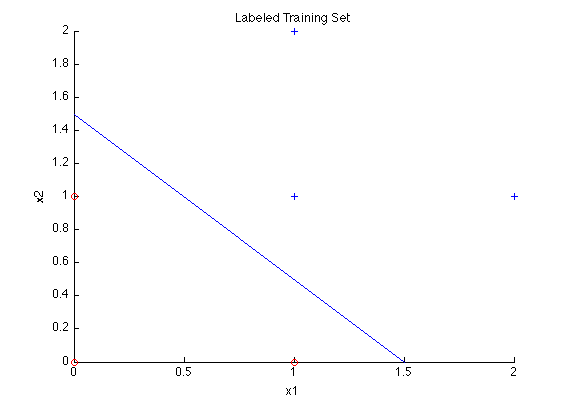
\includegraphics[width=0.7\textwidth]{SVMplot}
  \caption{Training set and optimal separating line}
\end{figure}

In this simple dataset it is clear that the classifier with the largest margin will pass through the points (0.5, 1) and (1, 0.5). 
Looking at the line we can see that the support vectors are (0, 1): -1, (1, 0): -1 and (1,1): +1. 
These points are all the same distance from the line.
As a result, it can be determined trigonometrically that the seperating margin is $\frac{1}{4}\sqrt{2}$


\end{document}
